\documentclass[journal]{vgtc}                     % final (journal style)
%\documentclass[journal,hideappendix]{vgtc}        % final (journal style) without appendices
%\documentclass[review,journal]{vgtc}              % review (journal style)
%\documentclass[review,journal,hideappendix]{vgtc} % review (journal style)
%\documentclass[widereview]{vgtc}                  % wide-spaced review
%\documentclass[preprint,journal]{vgtc}            % preprint (journal style)


%% Uncomment one of the lines above depending on where your paper is
%% in the conference process. ``review'' and ``widereview'' are for review
%% submission, ``preprint'' is for pre-publication in an open access repository,
%% and the final version doesn't use a specific qualifier.

%% If you are submitting a paper to a conference for review with a double
%% blind reviewing process, please use one of the ``review'' options and replace the value ``0'' below with your
%% OnlineID. Otherwise, you may safely leave it at ``0''.
\onlineid{0}

%% In preprint mode you may define your own headline. If not, the default IEEE copyright message will appear in preprint mode.
%\preprinttext{To appear in IEEE Transactions on Visualization and Computer Graphics.}

%% In preprint mode, this adds a link to the version of the paper on IEEEXplore
%% Uncomment this line when you produce a preprint version of the article 
%% after the article receives a DOI for the paper from IEEE
%\ieeedoi{xx.xxxx/TVCG.201x.xxxxxxx}

%% declare the category of your paper, only shown in review mode
\vgtccategory{Research}

%% please declare the paper type of your paper to help reviewers, only shown in review mode
%% choices:
%% * algorithm/technique
%% * application/design study
%% * evaluation
%% * system
%% * theory/model
\vgtcpapertype{application/design study}

%% Paper title.
\title{ExcavatorVR - Simulating an Excavator in Virtual Reality}

%% Author ORCID IDs should be specified using \authororcid like below inside
%% of the \author command. ORCID IDs can be registered at https://orcid.org/.
%% Include only the 16-digit dashed ID.
\author{%
  Sebastian Gradwohl*
}

\authorfooter{
  %% insert punctuation at end of each item
  \item
  	* Sebastian Gradwohl  is a Software Engineering Student of the University of Applied Sciences Upper Austria - Hagenberg

  	E-mail: s2310307057@fhooe.at
}

%% Abstract section.
\abstract{%
  This paper is focussed on the design and implementation of a fully simulated excavator-driving environment for the Oculus Rift-S. The Goal was to simulate the controls of a real excavator as accurately as possible.
}

%% Keywords that describe your work. Will show as 'Index Terms' in journal
%% please capitalize first letter and insert punctuation after last keyword
\keywords{Virtual Reality, Machine Controls}

% A teaser figure can be included as follows
\teaser{
  \centering
  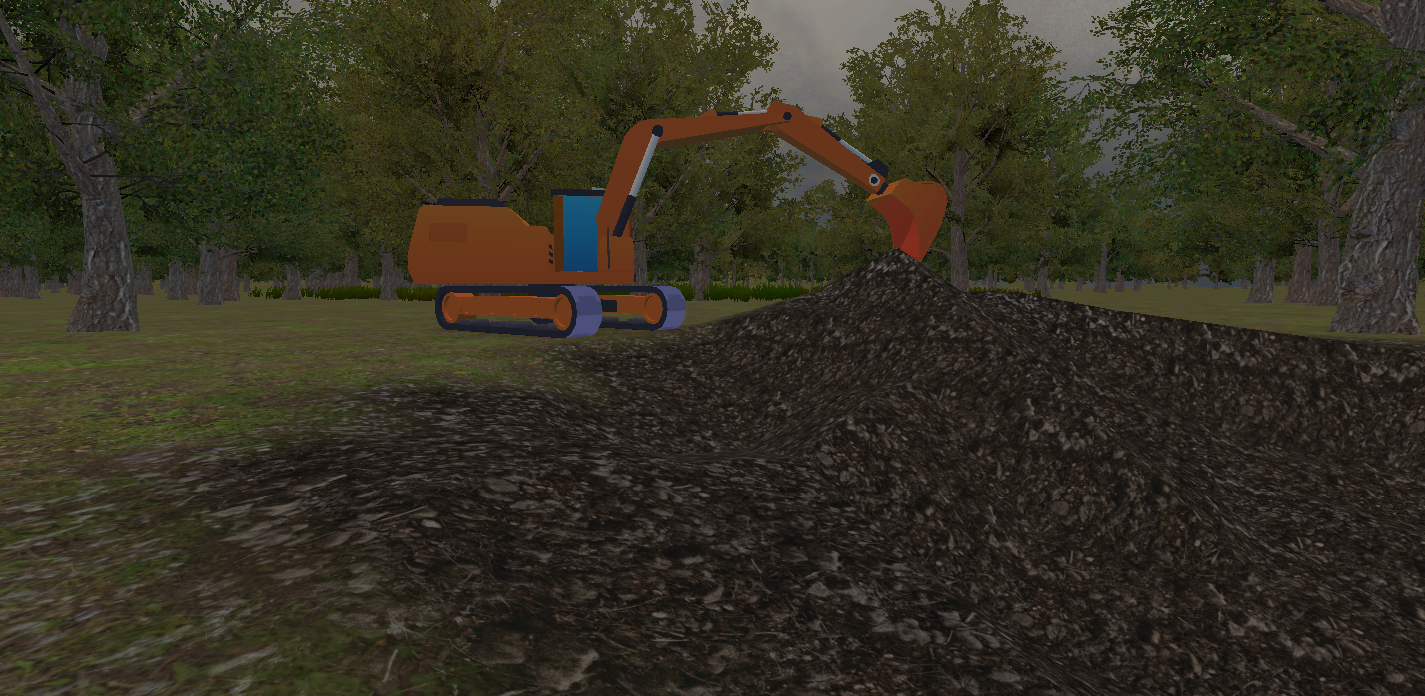
\includegraphics[width=\linewidth, alt={Outside View of the Excavator after digging out an area}]{ExcavatorOutsideView}
  \caption{%
  	An outside view from the excavator after a quick playtest to dig out a smaller area%
  }
  \label{fig:teaser}
}

%% Uncomment below to disable the manuscript note
\renewcommand{\manuscriptnotetxt}{}

%% Copyright space is enabled by default as required by guidelines.
%% It is disabled by the 'review' option or via the following command:
%\nocopyrightspace


%%%%%%%%%%%%%%%%%%%%%%%%%%%%%%%%%%%%%%%%%%%%%%%%%%%%%%%%%%%%%%%%
%%%%%%%%%%%%%%%%%%%%%% LOAD PACKAGES %%%%%%%%%%%%%%%%%%%%%%%%%%%
%%%%%%%%%%%%%%%%%%%%%%%%%%%%%%%%%%%%%%%%%%%%%%%%%%%%%%%%%%%%%%%%

%% Tell graphicx where to find files for figures when calling \includegraphics.
%% Note that due to the \DeclareGraphicsExtensions{} call it is no longer necessary
%% to provide the the path and extension of a graphics file:
%% 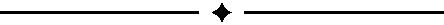
\includegraphics{diamondrule} is completely sufficient.
\graphicspath{{figs/}{figures/}{pictures/}{images/}{./}} % where to search for the images

%% Only used in the template examples. You can remove these lines.
\usepackage{tabu}                      % only used for the table example
\usepackage{booktabs}                  % only used for the table example
\usepackage{lipsum}                    % used to generate placeholder text
\usepackage{mwe}                       % used to generate placeholder figures

%% We encourage the use of mathptmx for consistent usage of times font
%% throughout the proceedings. However, if you encounter conflicts
%% with other math-related packages, you may want to disable it.
\usepackage{mathptmx}                  % use matching math font

\begin{document}

%%%%%%%%%%%%%%%%%%%%%%%%%%%%%%%%%%%%%%%%%%%%%%%%%%%%%%%%%%%%%%%%
%%%%%%%%%%%%%%%%%%%%%% START OF THE PAPER %%%%%%%%%%%%%%%%%%%%%%
%%%%%%%%%%%%%%%%%%%%%%%%%%%%%%%%%%%%%%%%%%%%%%%%%%%%%%%%%%%%%%%%

%% The ``\maketitle'' command must be the first command after the
%% ``\begin{document}'' command. It prepares and prints the title block.
%% the only exception to this rule is the \firstsection command#
\firstsection{Introduction}

\maketitle


%% \section{Introduction} %for journal use above \firstsection{..} instead
Over the years there have been many attempts trying to create training and demo simulators for different kinds of jobs. Virtual Reality provides an irreplacable opportunity to make the experience as realistic and easy to use as possible.
Many different industries are already creating such software and distributing it, either for their customers or for their own employees. 

Such software allows the users to train for a  job in a safe space where the risk of accidents can be severely reduced whilst the economical and health dangers surrounding these are minimized.

During the planning stage of this project, the severe lack of training software for the construction industry in particular really stuck out. 
Therefore, in this context, the decision was made to create a small training simulator for excavator operators. Excavators have a comparatively high complexity for their controls compared to other construction vehicles, due to the simultaneous handling of multiple joysticks and levers. 

Because of this, operators need alot of intuition and experience to use the machine effectively, which made this kind of vehicle the choice for this project.

\section{User Guide}

This project is designed to be played in a seated manner. The user is not supposed to change their position during the duration of the playsession. The chair should be placed in the middle of the playspace and should face to the front of the configured playspace of the HMDs software.

The user requires a HMD of their choice, but preferrably a Oculus Rift-S and one controller for each hand, which is compatible with their HMD.

\begin{figure}[tb]% specify a combination of t, b, p, or h for top, bottom, on its own page, or here
  \centering % avoid the use of \begin{center}...\end{center} and use \centering instead (more compact)
  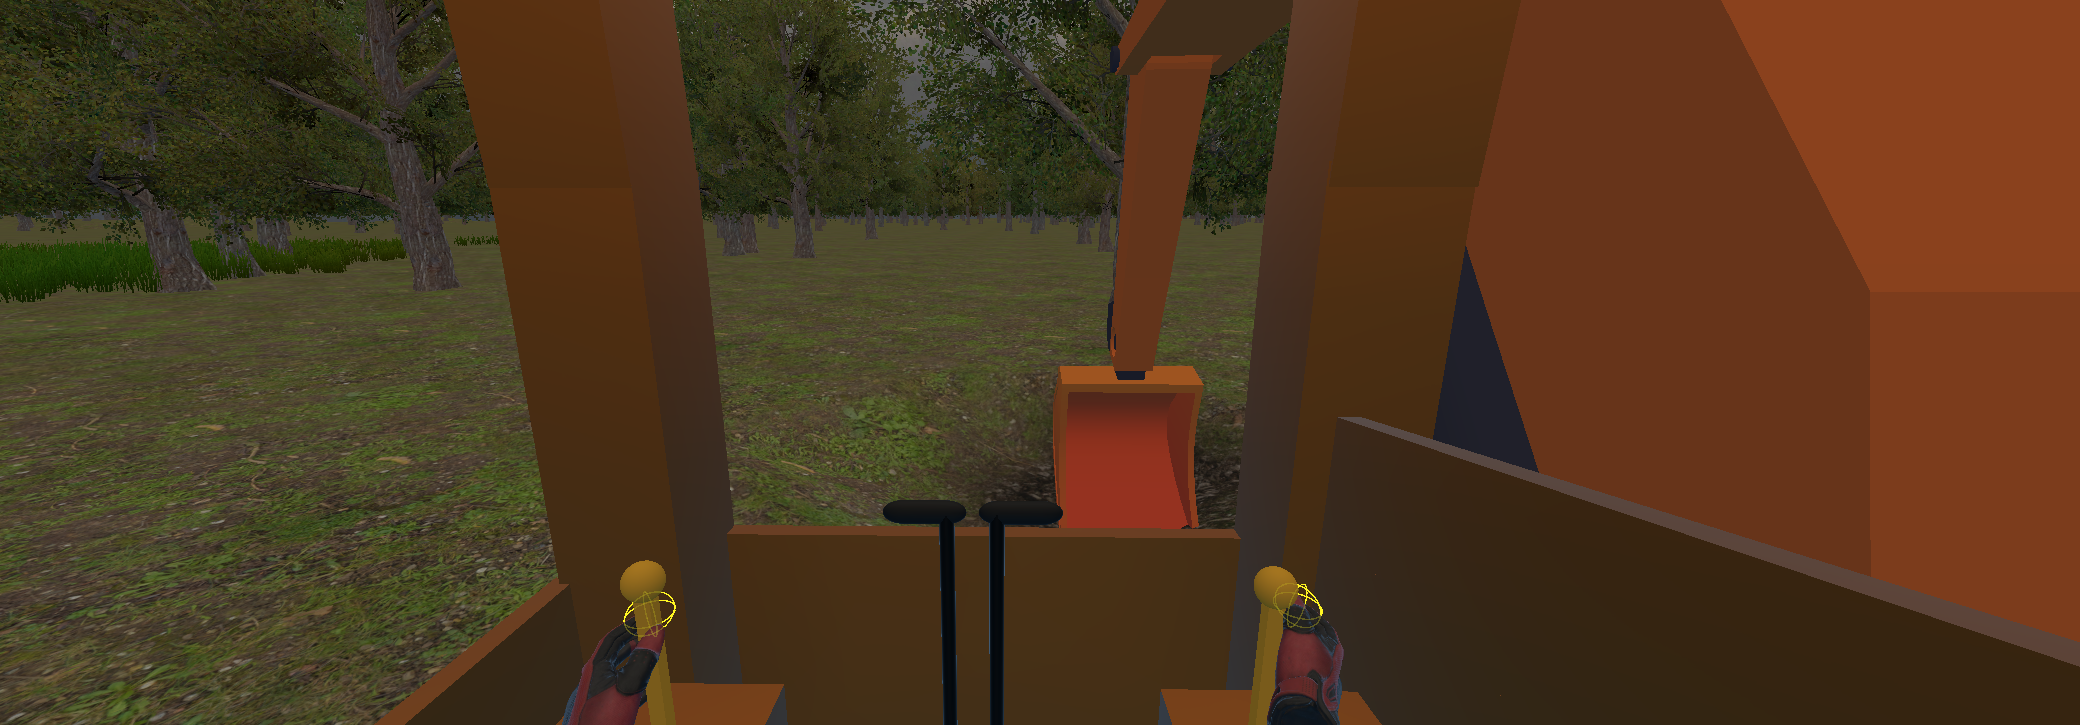
\includegraphics[width=\columnwidth, alt={The view from the cabin of a excavator. Each hand is on the joystick for controlling the vehicles arms and body}]{ExcavatorCabinView}
  \caption{%
  	The view of the player during his VR experience%
  }
  \label{fig:cabin_view}
\end{figure}

\subsection{First Steps}
After startup the user is immediately placed into the drivers seat of their excavator. On both sides next to the seat there are two yellow joysticks with a sphere on top of them, placed in a manner to make it natural for the user to grab them from a seated position. In front of the seat, right before the front window there are two additional black levers.

The Controls of the excavator are based on the ISO Standard 10968. This Standard defines the following controls for the excavator:

\begin{itemize}
  \item The left joystick tilting left causes the excavators upper body to swing left
  \item The left joystick tilting right causes the excavators upper body to swing right
  \item The left joystick tilting forward causes the excavators dipper, also known as stick boom, to move away from the excavators main body.
           The Stick Boom of the excavator is the second half of the excavators arm, connecting the main boom with the bucket.
  \item The left joystick tilting backwards causes the excavators stick boom, to move closer to the excavators main body.
  \item The right joystick tilting left causes the bucket of the excavator to curl in, therefore closing
  \item The right joystick tilting right causes the bucket of the excavator to curl out. Thereby allowing for the bucket to dump its contents
  \item The right joystick tilting forward causes the main boom and therefore the entire arm to go down
  \item The right joystick tilting backwards causes the main boom to go back up 
  \item The left lever in front of the seat defines the movement of the left track of the excavator. The further it gets tilted, the faster the track moves. If it gets tilted backwards, the track moves backwards instead.
  \item The right lever in front of the seat defines the movement of the right track of the excavator. The further it gets tilted, the faster the track moves. If it gets tilted backwards, the track moves backwards instead.
\end{itemize}

Theoretically there is a second standard for the controls, SAE J1814, inverting the main and stick booms controls compared to ISO 10968, but for this project in particular, the focus was put on the ISO standard.

The interaction is possible by hovering over whichever object should be selected with a hand and then pressing the HMD-controllers grip button. For most controllers this button is placed in a position, to naturally press it when gripping the controller more tightly. For the Track-Levers the forward or backward movement of the hand is translated into the lever moving forward or backwards. For the Joysticks a different methodology had to be found, due to the translation of 360° movement into a translatable rotation proved more difficult than first expected. Therefore the behavior for the joysticks was made to relay the rotation movement of the hand to the joystick. Due to the size of the joysticks being alot smaller compared to the levers, used for controlling the tracks,l this solution works quite well. The smaller size of the joystick would make moving ones hand further away and still controlling the joystick rather unrealistic and unintuitive in comparison to the larger Track-Levers.

\section{Design}

While a VR Project comes with a lot of weaknesses inherent to the nature of the current hardware, it also provides many possibilities and strengths which are impossible to reproduce with other forms of media.
The goal of this project was to use as many of the strengths whilst avoiding or mitigating the many pitfalls alot of VR software is commonly affected by, such as motion sickness or high latency with the interactions


\subsection{Keeping it simple}

Freedom often leads to confusion. Therefore the goal was to streamline the user experience in a way, where the user is not overwhelmed and neither completely left to their own devices. This is managed through a few smaller systems and design decisions, which are explained in the next chapters.


\subsection{Seated like in reality}

Due to the focus being on simulating an excavator operators experience the decision was made to keep the user in the same location at all times. Whilst movement is still allowed, to enable the user to, for example, look out of the window of the vehicle. There is no incentive to leave the seated area.

This decision also avoids alot of issues concerning motion sickness. Due to the user being in a seated position and the velocity of the excavator being rather slow by nature, moving with the excavator is not nausea inducing and should therefore make the simulation alot more accessible to users with less to no experience with Virtual Reality.


\begin{figure}[tb]% specify a combination of t, b, p, or h for top, bottom, on its own page, or here
  \centering % avoid the use of \begin{center}...\end{center} and use \centering instead (more compact)
  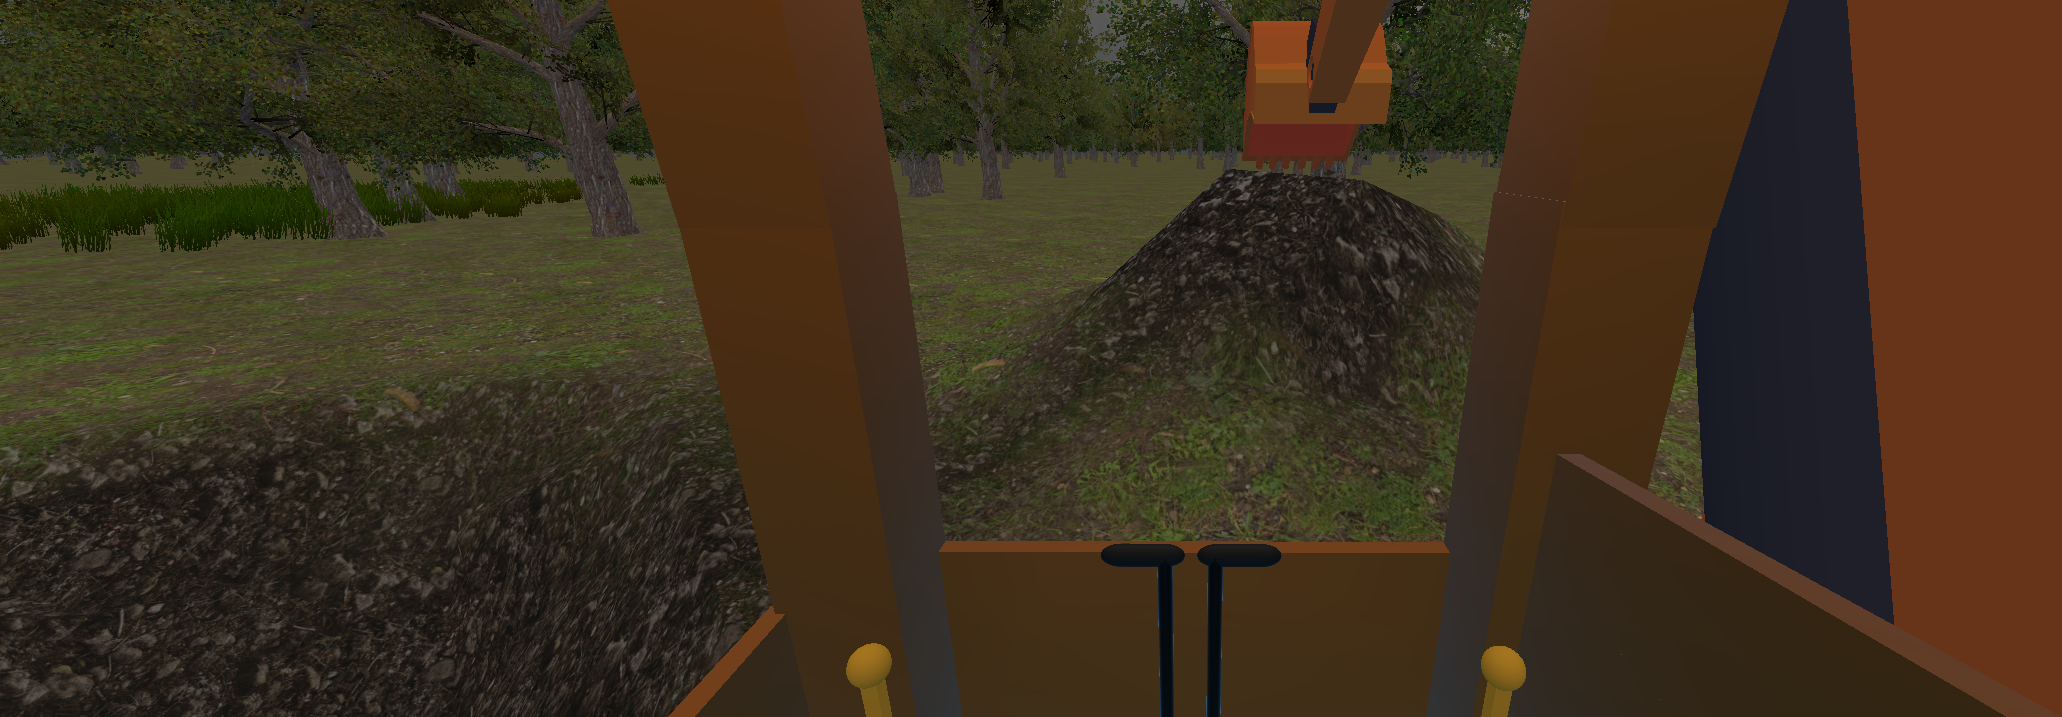
\includegraphics[width=\columnwidth, alt={The view from the cabin of a excavator. On one side there is a smaller hole, next to it lies a small heap of material, suggesting the excavator dug it out. the shovel is placed neatly on top of the heap}]{GroundDeformation}
  \caption{%
  	The view from the cabin after digging out a small hole and dumping material to create a small heap%
  }
  \label{fig:cabin_view}
\end{figure}

\subsection{The world confirms the excavators existance}

One important aspect of the simulation was of course the excavator buckets behavior. After all, getting a hang of the controls to move each component of an excavator effectively is only the beginning. Due to this, it was essential to implement the most common task of excavators: The movement of material through an area by digging it away and dumping it somewhere else.

This could be achieved by enabling the shovel to interact with the surrounding terrain of the excavator, allowing for it to create holes when digging and to dump material when opening the shovel over the terrain.


\section{Implementation}
For this project there are both generic scripts and vehicle-control scripts. Whilst the generic scripts can be partially reused in other usecases the contents of the vehicle-controls are exclusively usable for vehicle controls.

The logic for moving the track of the excavator was abstracted into its own class. In case the program is to be expanded in the future with further track-based vehicles, the class could be used as a basis.


\subsection{Track Lever Spring behavior} \label{trackLeverSpringBehavior}
This script is used for the track-levers. In reality, after letting go of the lever, it slowly moves back to its initial position. After some initial attempts to accomplish this behavior using the spring-feature of the Unity-Default Hinge-Joints, it was discovered, that due to the levers being kinetic rigidbodies, the spring behavior would not work properly. 

Because of this, the behavior had to be implemented by hand. The created script also allows for the hand to snap to the lever upon grabbing it and lets go of it, if the grab-interaction ends.

To smooth out the spring-functionality, the rotation of the lever is changed with linear interpolation.


\subsection{Terrain Manipulation}

The logic for this feature was based on the assumption of it only being used on an object, which points at the terrain whenever it wishes to manipulate it. 
An example for this would be a Unity GameObject placed right at the blade of an excavators bucket.

To determine, if the shovel is currently interacting with the terrain a raycast is sent out from the object, the script is used on. If the raycast hits the terrain and the hit was within a certain distance it remembers the distance to choose the terraforming action. From here the behavior splits up in multiple paths:

\begin{itemize}
  \item If the raycast distance was incredibly short, the script assumes the shovel is currently touching the terrain, therefore it starts lowering the terrain around the area the raycast hit.
  \item The raycast had a measurable distance, but the bucket is currently not opened into the direction of the ground, therefore any further behavior is stopped for this frame, since the bucket is not currently dumping any material
  \item The raycast had a measurable distance and the bucket is currently open. This suggests the excavator is currently dumping material. Therefore the terrain gets raised around the raycast-hit-position.
\end{itemize}

To manipulate the terrain the script must begin by translating the world position of the raycast-target into the local position of the terrain. 

After that is completed, the heightmap of the terrain around the calculated local position of the raycast-target gets adjusted, either raised or lowered by a fixed value. To keep the increase independant of the framerate the constant manipulation-strength gets multiplied by the time difference from the last frame to the current one.

Additionally to provide additional feedback for the user, the texture of manipulated terrain changes to a dirt-like texture, to make smaller terraforming-changes stick out a bit more.

\begin{figure}[h]% specify a combination of t, b, p, or h for top, bottom, on its own page, or here
  \centering % avoid the use of \begin{center}...\end{center} and use \centering instead (more compact)
  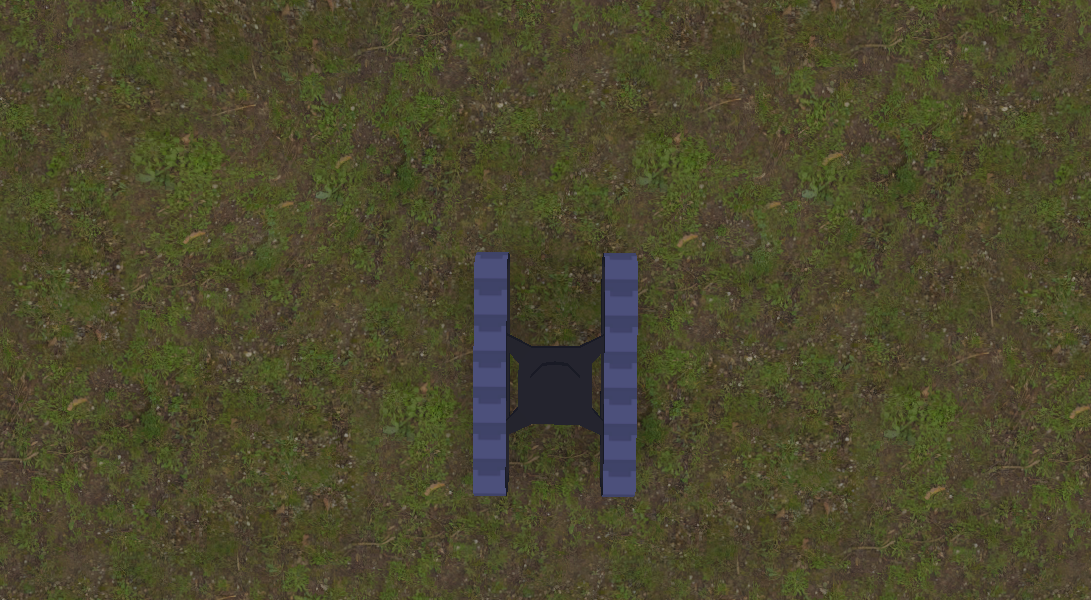
\includegraphics[width=0.45\textwidth, alt={A Top-Down View of the track-base of the excavator with a few circles and radius showing the different values required for calculating the skid steering rotation}]{TrackBase}
  \caption{%
  	A small sketch showing the different values required for the skid steering calculation visually%
  }
  \label{fig:skid_steering_sketch}
\end{figure}
\subsection{Track Movement}

For the Logic of the track movement, the algorithm requires two lever gameobjects whose rotation is then used to calculate the speed for both of the tracks. This speed is then used to calculate the rotation and distance to move the vehicle.

These levers are then checked for their angle on every frame and the angle gets converted into a relative speed value with their max-angle being the maximum speed and an angle of 0 being a speed of 0.

In case both levers have a similar rotation a straight forward movement can be achieved, Otherwise the deviation from the course needs to be calculates. For that the radius of the inner track of the rotation needs to be calculated. This can be achieved by taking the width between both sides of the vehicle and dividing it by the relative speed of the fast to the slow track - 1. Afterwards the speed of the outer track needs to be divided through the calculated radius with the width between both sides of the vehicle added to it. This calculates the degree value on how far the excavator needs to be rotated.

From that rotation value the algorithm can then also calculate the distance the vehicle is supposed to move forward to simulate the different rotation center-point, by multiplying it with the sinus-value

\subsection{Translating hand rotation to joystick rotation}

For this logic a few requirements had to be considered whenever this behavior should be used:

\begin{itemize}
  \item The hand rotation should only be copied to the joystick if the user is actually grabbing the joystick
  \item Only the currently gripped joystick should be affected and only by the rotation of the currently interacting hand.
  \item If both hands grip two joysticks, the translation needs to work for both of them simultaneously
\end{itemize}

Whenever a joystick is gripped, the rotation of the current hand is collected and compared with the last update of the joysticks rotation. The difference of the rotation is then applied to the joystick. Once again, a similar functionality to the track-lever spring behavior, from subsection \ref{trackLeverSpringBehavior} on page \pageref{trackLeverSpringBehavior}, is implemented here, with the only difference being, that this script considers both the x and y axis.

With this translation the z-axis  is deliberately kept consistent to keep the later translation in the excavator behavior simpler.

\subsection{Translating joystick rotation into excavator movements}

For this translation each axis of the joysticks are handled seperately. The relative speed is calculated by the angle of the joystick and it is then used to add or reduce the current rotation-value of the axis to be manipulated for each component of the excavator. In the case of the stick-boom and for the bucket, the velocity needs to be inverted, as a forward movement is seen as a positive rotation change, but the rotation should actually change into the negative.

To avoid any motion sickess during the excavator body swing or any snappy reactions of the excavator the movement needs to be smooth. The change of the rotation is therefore once again applied with a linear interpolation to smooth out the movement.

\section{Future Improvements}

As of now the projects serves as a nice proof of concept and a small tech demo. Therefore there are alot of features to be added or further polished.

One of those features would be the correct placement of the hands when grabbing the track-levers. Currently they snap to the basis of the lever, sadly some experimentation with the attachment offset of the hand assets did not prove successful, but it would prove to be a great improvement.

Currently there is also the missing logic of a bucket fill-state, currently you can remove and dump infinite material from the bucket, a limit on how much the bucket can remove before it needs to be dumped and a fill-state for the bucket with visualization would surely improve the realism and make for a great improvement

Other than that this project provides a great basis to implement further vehicles to drive, like a dumper, a dozer or maybe even a crane.

%% if specified like this the section will be omitted in review mode
\acknowledgments{%
	The author wishes to thank Florian Rittberger and Nico Kern for proofreading and providing feedback for the document.
}


\bibliographystyle{abbrv-doi-hyperref}
%\bibliographystyle{abbrv-doi-hyperref-narrow}
%\bibliographystyle{abbrv-doi}
%\bibliographystyle{abbrv-doi-narrow}

\bibliography{template}


\end{document}

